\documentclass[10pt,a4paper,notitlepage]{article}
\usepackage[utf8]{inputenc}
\usepackage[french]{babel}
\usepackage[T1]{fontenc}
\usepackage{mathtools}
\usepackage[left=2cm,right=2cm,top=2cm,bottom=2cm]{geometry}
\usepackage{graphicx}
\usepackage{float}
\usepackage{subcaption}
\usepackage{tikz}

\usepackage{siunitx}
\usepackage{numprint}

\addto{\captionsfrench}{\renewcommand{\abstractname}{Introduction}}

\author{Pierre-Antoine Comby}
\title{TP2 : Commande d'un bras à liaison flexible par bouclage linéarisant}

\usepackage{enumitem}
\setlist[itemize]{label=\textbullet}

%ensembles usuels
\newcommand{\R}{\mathbb{R}}
\newcommand{\C}{\mathbb{C}}
\newcommand{\N}{\mathbb{N}}
\newcommand{\Z}{\mathbb{Z}}

\newcommand{\K}{\mathbb{K}}
\newcommand{\M}{\mathcal{M}}
\newcommand{\Lin}{\mathcal{L}}
\newcommand{\Img}{\text{Im}}
\newcommand{\Ker}{\text{Ker}}
\newcommand{\A}{\text{A}}
\newcommand{\B}{\text{B}}
\newcommand{\fromatob}{\A\to\B}

\DeclareFontFamily{U}{wncy}{}
\DeclareFontShape{U}{wncy}{m}{n}{<->wncyr10}{}
\DeclareSymbolFont{mcy}{U}{wncy}{m}{n}
\DeclareMathSymbol{\Sh}{\mathord}{mcy}{"58}

%relations

\newcommand{\eqv}{\Leftrightarrow}
\newcommand{\tr}{{}^t\! }

\DeclareMathOperator*{\equals}{=}

\newcommand{\limfty}[1]{\xrightarrow[#1 \to +\infty]{}}
\newcommand{\simfty}{\underset{+\infty}{\sim}}

\newcommand{\intinfty}{\int_{-\infty}^{+\infty}}

\renewcommand{\d}{\mathrm{d}}
\newcommand{\dd}[2]{\frac{\d #1}{\d #2}}
\newcommand{\ddd}[2]{\frac{\d^2 #1}{\d {#2}^2}}
\newcommand{\dr}[2]{\frac{\partial #1}{\partial #2}}
\newcommand{\divv}{\text{div}}
\newcommand{\grad}{\text{grad}}
\newcommand{\et}{\quad\text{ et }\quad}
\newcommand{\avec}{\quad\text{ avec }\quad}
\newcommand{\sinon}{\quad\text{ sinon }\quad}
\newcommand{\skzi}{\sum_{k=-\infty}^{+\infty}}
%Macros mieux :)
\newcommand{\chimie}[1]{$\mathrm{#1}$}
\newcommand{\chimiecite}[1]{\[\mathrm{#1}\]}
\newcommand{\nchim}{\mathit{n}}
\newcommand{\xchim}{\mathit{x}}
\renewcommand{\unit}[1]{~\mathrm{#1}}
\renewcommand{\d}{\mbox{d}}
\newcommand{\deriv}[2][]{\frac{\d#1}{\d#2}}
\newcommand{\derivp}[2][]{\frac{\partial#1}{\partial#2}}
\newcommand{\derivpp}[2][]{\frac{\partial^2#1}{\partial#2^2}}

\newcommand{\NA}{\mathcal{N}_A}% Avogadro
\newcommand{\e}{\text{e}}
\newcommand{\sinc}{\text{sinc}}

\newcommand{\fonct}[4]{%
\left\lbrace \begin{array}{l}
{#1}\longrightarrow {#2} \\
{#3}\longmapsto {#4}
\end{array}\right.}
\newcommand{\vect}[1]{%
  \begin{bmatrix}
    #1
  \end{bmatrix}
}

\makeatletter

\@ifpackageloaded{circuitikz}{%
\tikzset{every picture/.style={execute at begin picture={%
   \shorthandoff{:;!?};}}}}{}

\@ifpackageloaded{stmaryrd}{%
\newcommand{\entint}[1]{\llbracket #1 \rrbracket}}{}
\@ifpackageloaded{siunitx}{%
%\newcommand{\gdr}[3]{\ensuremath{#1 = }\SI{#2}{#3}}

}{}
\@ifpackageloaded{listings}{%
\usepackage{xcolor}

\AtBeginDocument{%
\lstset{
    language=Python,
    basicstyle=\ttfamily\small,
    aboveskip={1.0\baselineskip},
    belowskip={1.0\baselineskip},
    columns=fixed,
    extendedchars=true,
    breaklines=true,
    tabsize=4,
    prebreak=\raisebox{0ex}[0ex][0ex]{\ensuremath{\hookleftarrow}},
    frame=lines,
    showtabs=false,
    showspaces=false,
    showstringspaces=false,
    keywordstyle=\color[rgb]{0.627,0.126,0.941},
    commentstyle=\color[rgb]{0.133,0.545,0.133},
    stringstyle=\color[rgb]{01,0,0},
    numbers=left,
    numberstyle=\small,
    stepnumber=1,
    numbersep=10pt,
    captionpos=t,
    literate={{á}{{\'a}}1 {é}{{\'e}}1 {í}{{\'i}}1 {ó}{{\'o}}1 {ú}{{\'u}}1
  {Á}{{\'A}}1 {É}{{\'E}}1 {Í}{{\'I}}1 {Ó}{{\'O}}1 {Ú}{{\'U}}1
  {à}{{\`a}}1 {è}{{\`e}}1 {ì}{{\`i}}1 {ò}{{\`o}}1 {ù}{{\`u}}1
  {À}{{\`A}}1 {È}{{\'E}}1 {Ì}{{\`I}}1 {Ò}{{\`O}}1 {Ù}{{\`U}}1
  {ä}{{\"a}}1 {ë}{{\"e}}1 {ï}{{\"i}}1 {ö}{{\"o}}1 {ü}{{\"u}}1
  {Ä}{{\"A}}1 {Ë}{{\"E}}1 {Ï}{{\"I}}1 {Ö}{{\"O}}1 {Ü}{{\"U}}1
  {â}{{\^a}}1 {ê}{{\^e}}1 {î}{{\^i}}1 {ô}{{\^o}}1 {û}{{\^u}}1
  {Â}{{\^A}}1 {Ê}{{\^E}}1 {Î}{{\^I}}1 {Ô}{{\^O}}1 {Û}{{\^U}}1
  {œ}{{\oe}}1 {Œ}{{\OE}}1 {æ}{{\ae}}1 {Æ}{{\AE}}1 {ß}{{\ss}}1
  {ű}{{\H{u}}}1 {Ű}{{\H{U}}}1 {ő}{{\H{o}}}1 {Ő}{{\H{O}}}1
  {ç}{{\c c}}1 {Ç}{{\c C}}1 {ø}{{\o}}1 {å}{{\r a}}1 {Å}{{\r A}}1
  {€}{{\euro}}1 {£}{{\pounds}}1 {«}{{\guillemotleft}}1
  {»}{{\guillemotright}}1 {ñ}{{\~n}}1 {Ñ}{{\~N}}1 {¿}{{?`}}1}
}
\lstset{language=Matlab,%
    %basicstyle=\color{red},
    breaklines=true,%
    morekeywords={matlab2tikz},
    keywordstyle=\color{blue},%
    morekeywords=[2]{1}, keywordstyle=[2]{\color{black}},
    identifierstyle=\color{black},%
    stringstyle=\color{mylilas},
    commentstyle=\color{mygreen},%
    showstringspaces=false,%without this there will be a symbol in the places where there is a space
    numbers=left,%
    numberstyle={\tiny \color{black}},% size of the numbers
    numbersep=9pt, % this defines how far the numbers are from the text
    emph=[1]{for,end,break},emphstyle=[1]\color{red}, %some words to emphasise
    literate=
    {á}{{\'a}}1 {é}{{\'e}}1 {í}{{\'i}}1 {ó}{{\'o}}1 {ú}{{\'u}}1
    {Á}{{\'A}}1 {É}{{\'E}}1 {Í}{{\'I}}1 {Ó}{{\'O}}1 {Ú}{{\'U}}1
    {à}{{\`a}}1 {è}{{\`e}}1 {ì}{{\`i}}1 {ò}{{\`o}}1 {ù}{{\`u}}1
    {À}{{\`A}}1 {È}{{\'E}}1 {Ì}{{\`I}}1 {Ò}{{\`O}}1 {Ù}{{\`U}}1
    {ä}{{\"a}}1 {ë}{{\"e}}1 {ï}{{\"i}}1 {ö}{{\"o}}1 {ü}{{\"u}}1
    {Ä}{{\"A}}1 {Ë}{{\"E}}1 {Ï}{{\"I}}1 {Ö}{{\"O}}1 {Ü}{{\"U}}1
    {â}{{\^a}}1 {ê}{{\^e}}1 {î}{{\^i}}1 {ô}{{\^o}}1 {û}{{\^u}}1
    {Â}{{\^A}}1 {Ê}{{\^E}}1 {Î}{{\^I}}1 {Ô}{{\^O}}1 {Û}{{\^U}}1
    {œ}{{\oe}}1 {Œ}{{\OE}}1 {æ}{{\ae}}1 {Æ}{{\AE}}1 {ß}{{\ss}}1
    {ű}{{\H{u}}}1 {Ű}{{\H{U}}}1 {ő}{{\H{o}}}1 {Ő}{{\H{O}}}1
    {ç}{{\c c}}1 {Ç}{{\\cite{}  C}}1 {ø}{{\o}}1 {å}{{\r a}}1 {Å}{{\r A}}1
    {€}{{\euro}}1 {£}{{\pounds}}1 {«}{{\guillemotleft}}1
    {»}{{\guillemotright}}1 {ñ}{{\~n}}1 {Ñ}{{\~N}}1 {¿}{{?`}}1
  }
}}{}
\makeatother

\renewcommand{\R}{\mathbb{R}}
\renewcommand{\Z}{\mathbb{Z}}
\renewcommand{\vec}{\overrightarrow}
\usepackage{minted}
\begin{document}
\maketitle
\section{Modélisation}
\paragraph{Prépa.1}
\begin{itemize}
\item On applique le PFD au chariot \{1\}de masse $M_c$:
\begin{equation}
  M_c\vec{a_{\{1\}}} = \vec{F}+\vec{T}-C_d\vec{v_{\{1\}}}+M_c\vec{g}
\end{equation}
Soit en projetant:
\begin{equation}
  M_c \ddot{d} = F+T\sin(\theta)-C_d\dot{d}
\end{equation}
\item On fait de meme pour la masse pendulaire \{2\} $m$:
\begin{equation}
  m \vec{a_{\{2\}}} = -\vec{T} +m \vec{g}
\end{equation}
et il vient directement:
\begin{equation}
  \begin{cases}
    m\ddot{x} = -T\sin(\theta)\\
    m\ddot{z} = -T\cos(\theta)+mg
  \end{cases}
\end{equation}
\item et un théorème du moment cinétique sur l'arbre donne (avec $\alpha$ angle du tambour par rapport au chariot):
  \begin{equation}
    J\ddot{\alpha} = -C +bT-C_r \dot{\alpha}
  \end{equation}
  soit :
  \begin{equation}
    J \frac{\ddot{r}}{b} = -C+bT -C_r \frac{\dot{r}}{b}
  \end{equation}
\end{itemize}
\paragraph{Prépa.2}
Comme $b\ll r$ on a :
\begin{equation}
  \begin{cases}
    x = r\sin\theta+d\\
    z = r\cos\theta
  \end{cases}
\end{equation}
soit :
\begin{equation}
  \begin{cases}
    \dot{x} = \dot{r}\sin\theta + r\dot{\theta}\cos\theta +\dot{d}\\
    \dot{z} = \dot{r}\cos\theta -r\dot{\theta}\sin\theta
  \end{cases}
  \quad\text{ et }\quad
  \begin{cases}
    \ddot{x} = \ddot{r}\sin\theta+2\dot{r}\dot{\theta}\cos\theta+r\ddot{\theta}\cos\theta- r\dot{\theta}^2\sin\theta+\ddot{d}\\
    \ddot{z} = \ddot{r}\cos\theta-2\dot{r}\dot{\theta}\sin\theta-r\ddot{\theta}\sin\theta-r\dot{\theta}^2\cos\theta
  \end{cases}
\end{equation}
\paragraph{Prépa.3} en remplacant dans le système (1) donné dans l'énoncé on trouve:
\begin{equation}
  \begin{cases}
    m(
    \ddot{r} \sin\theta+2\dot{r}\dot{\theta}\cos\theta+r\ddot{\theta}\cos\theta-r\dot{\theta}^2\sin\theta+\ddot{d}
    ) &=-T\sin\theta\\
    m(
    \ddot{r}\cos{\theta}-2\dot{r}\dot{\theta}\sin\theta-r\ddot{\theta}\sin\theta-r\dot{\theta}^2\cos\theta
    ) &= - T\cos\theta+ mg
  \end{cases}
\end{equation}
A partir des identités trigonométrique on a :
\begin{equation}
  \begin{cases}
    m\ddot{r} &= - m\ddot{d}\sin\theta+mr\dot{\theta}^2 -T + mg \cos{\theta}\\
    r \ddot{\theta} &= -\ddot{d}\cos\theta-2\dot{r}\dot{\theta}-g\sin\theta 
  \end{cases}
\end{equation}
\paragraph{Prépa.4}
Des équations précédentes on en déduit le modèle d'état( en remplacant l'expression de $T$ par celle déduite de la prépa.3):
\begin{equation}
  \begin{cases}
    M_c\ddot{d} &= F +T \sin\theta-C_d\dot{d}\\
    r\ddot{\theta} &= -\ddot{d}\cos\theta-2\dot{r}\dot{\theta}-g\sin(\theta)\\
    (m+\frac{J}{b^2})\ddot{r} = -\frac{C}{b}-\frac{C_r\dot{r}}{b^2}-m\ddot{d}\sin\theta-mr\dot{\theta}^2+mg\cos{\theta}
  \end{cases}
\end{equation}

\paragraph{Prépa.5}
On linéarise autour de $d=D$,$r=R$,$\theta=0$, $T=mg$,$F=0$,$C=mbg$:
\begin{equation}
    \begin{cases}
M_{c}(\Delta d+D) &=(\Delta F)+T \sin (\Delta \theta)-C_{d}(\Delta d+D) \\(\Delta r+R)(\Delta \theta) &=-(\Delta d+D) \cos (\Delta \theta)-2(\Delta r+R)(\Delta \theta)-g \sin (\Delta \theta) \\\left(m+\frac{J}{b^{2}}\right)(\Delta r+R) &=-\frac{\Delta C+m g b}{b}-\frac{C_{r}(\Delta r+R)}{b^{2}}-m(\Delta d+D) \sin (\Delta \theta)-m(\Delta r+R)(\Delta \theta)^{2}+m g \cos (\Delta \theta)
\end{cases}
\end{equation}
En faisant une approximation au 1er ordre on a:
\begin{equation}
  \begin{cases}
    M_{c} \Delta d &=\Delta F+m g \Delta \theta-C_{d} \Delta d \\
    R \Delta \theta+\Delta d &=-g \Delta \theta \\
    \left(m+\frac{J}{b^{2}}\right) \ddot{\Delta r} &=-\frac{\Delta C+m g b}{b}-\frac{C_{r} \Delta r}{b^{2}}-m g \Delta \theta
  \end{cases}
  \implies
  \begin{cases} M_{c} \ddot{\Delta} d &=\Delta F+m g \Delta \theta-C_{d} \dot{\Delta} d \\
    R \Delta \theta+\Delta d &=-g \Delta \theta \\
    \left(m+\frac{J}{b^{2}}\right) \ddot{\Delta r} &=-\frac{\Delta C}{b}-\frac{C_{r} \Delta r}{b^{2}}
  \end{cases}
\end{equation}
On en deduit le modèle d'état linéarisé:
\[
  \deriv{t}\vect{\Delta d \\ \Delta r \\ \Delta\theta \\ \dot{\Delta d}\\ \dot{\Delta r}\\ \dot{\Delta \theta}} = 
  \left[ \begin{array}{cccccc}
           {0} & {0} & {0} & {1} & {0} & {0} \\
           {0} & {0} & {0} & {0} & {1} & {0} \\
           {0} & {0} & {0} & {0} & {0} & {1} \\
           {0} & {0} & {\frac{m g}{M_{c}}} & {-\frac{C_{d}}{M_{c}}} & {0} & {0} \\
           {0} & {0} & {0} & {0} & {-\frac{C_{r}}{J+m b^{2}}} & {0} \\
           {0} & {0} & {-\left(1+\frac{m}{M c}\right) \frac{g}{R}} & {\frac{C_{d}}{R M_{c}}} & {0} & {0}
         \end{array}\right] \cdot
       \left[ \begin{array}{c}{\Delta d} \\ {\Delta r} \\ {\Delta \theta} \\ {\Delta d} \\ {\Delta r} \\ {\Delta \theta}\end{array}\right]+
       \left[ \begin{array}{ccc}{0} & {0} \\ {0} & {0} \\ {0} & {0} \\ {\frac{1}{M_{c}}} & {0} \\ {0} & {-\frac{1}{\frac{J}{b}+m b^{2}}} \\ {-\frac{1}{R M_{c}}} & {0}\end{array}\right]
       \cdot \left[ \begin{array}{c}{\Delta F} \\ {\Delta C}\end{array}\right]
\]

\section{Commande linéaire}
\paragraph{Manip.1}
Dans le cas linéaire on construit la matrce de Kallman :
\[
  \mathcal{C} = \vect{B & AB & A^2B & A^5B }
\]
avec la fonction matlab \texttt{rank(Com)} on vérifie que le système est bien commandable.
\begin{minted}{matlab}
  A = [0 0 0 1 0 0 ; 
     0 0 0 0 1 0 ; 
     0 0 0 0 0 1 ; 
     0 0 m*g/Mc -Cd/Mc 0 0 ; 
     0 0 0 0 -Cr/(b^2*(J/b^2+m)) 0 ; 
     0 0 -g/R*(1+m/Mc) Cd/(Mc*R) 0 0];
B = [0 0 ; 
     0 0 ;
     0 0 ;
     1/Mc 0 ;
     0 -1/(b*(J/b^2+m)) ;
     -1/(R*Mc) 0 ];
Com = [B A*B A^2*B A^3*B A^4*B A^5*B];
rank(Com)
\end{minted}
On a un rang de 6, le système linéaire est bien commandable.
\paragraph{Manip.2}
avec la fonction \texttt{damp(eig(A))} on trouve les valeurs propres et constantes de temps de la matrice d'état
\begin{table}[H]
  \centering
  \begin{tabular}[t]{llll}
  \hline
  {\bf Pole}                 & {\bf Damping}   & {\bf Time Constant}  &            \\
\hline
                       &           & {(rad/TimeUnit)} & {(TimeUnit)} \\   
  
  0.00e+00             & -1.00e+00 & 0.00e+00       & Inf        \\
 -1.82e-04 + 1.48e+00i & 1.23e-04  & 1.48e+00       & 5.50e+03   \\ 
 -1.82e-04 - 1.48e+00i & 1.23e-04  & 1.48e+00       & 5.50e+03   \\ 
 -3.64e-03             & 1.00e+00  & 3.64e-03       & 2.75e+02   \\ 
  0.00e+00             & -1.00e+00 & 0.00e+00       & Inf        \\
  -1.54e-01             & 1.00e+00  & 1.54e-01       & 6.50e+00   \\
  \hline
\end{tabular}

\caption{Valeur propre et pulsation caractéristique}
\end{table}
On a donc la pulsation propre du système : $\omega_0$= \SI{1.48}{rad/s}. On choisi alors d'imposer les poles suivant, (d'après le cahier des charges) en ammortissant le pole double conjugué principal:
\[
  p_{1,2} = \omega_0(\xi\pm j \sqrt{1-\xi^2}) = 1.48(0.5\pm \sqrt{1-0.5^2})
\]
\begin{minted}{matlab}
  
vprA = damp(eig(A)); % valeur propres de A 
omega0 = vprA(2);
xi = 0.5
i=complex(0,1);
p1 = omega0*(xi+ i *sqrt(1-xi^2));
p2 = omega0*(xi- i *sqrt(1-xi^2));
p = [-2 -2.5 -3 -4 p1 p2];

K = place(A,B,p)

\end{minted}
\[K = 10^{5}\cdot
\begin{bmatrix}
  
    0.4288 & 0.1360  & 2.2614  & 0.0215 & 0.0506  & -0.9539 \\
   -0.0035 & -0.0261 & -0.0026 & 0.0019 & -0.0182 & 0.0195  \\

\end{bmatrix}\]
\paragraph{Manip.3}
Pour le terme de précommande, si l'on veux un gain statique unitaire, il faut\footnote{cf UE 421}:
\[
  \eta =\frac{-1}{C_1(A-BK)^{-1}B_1} = 4.1039. 10^{4}
\]
Avec $C_1$ et  $B_1$ lignes et colonnes des matrices $C$ et $B$ propre à $\Delta d$
\paragraph{Manip.4} L'ajout d'une composante intégrale va rendre notre système précis. On construit alors la fonction de transfert grace à MATLAB:
\begin{minted}{matlab}
  sys = ss( A-B*K,B(:,2),C(2,:), 0 );
  H = tf(sys);
  bode(H);
\end{minted}
On obtient le diagramme de bode suivant:
\begin{figure}[ht]
  \centering
  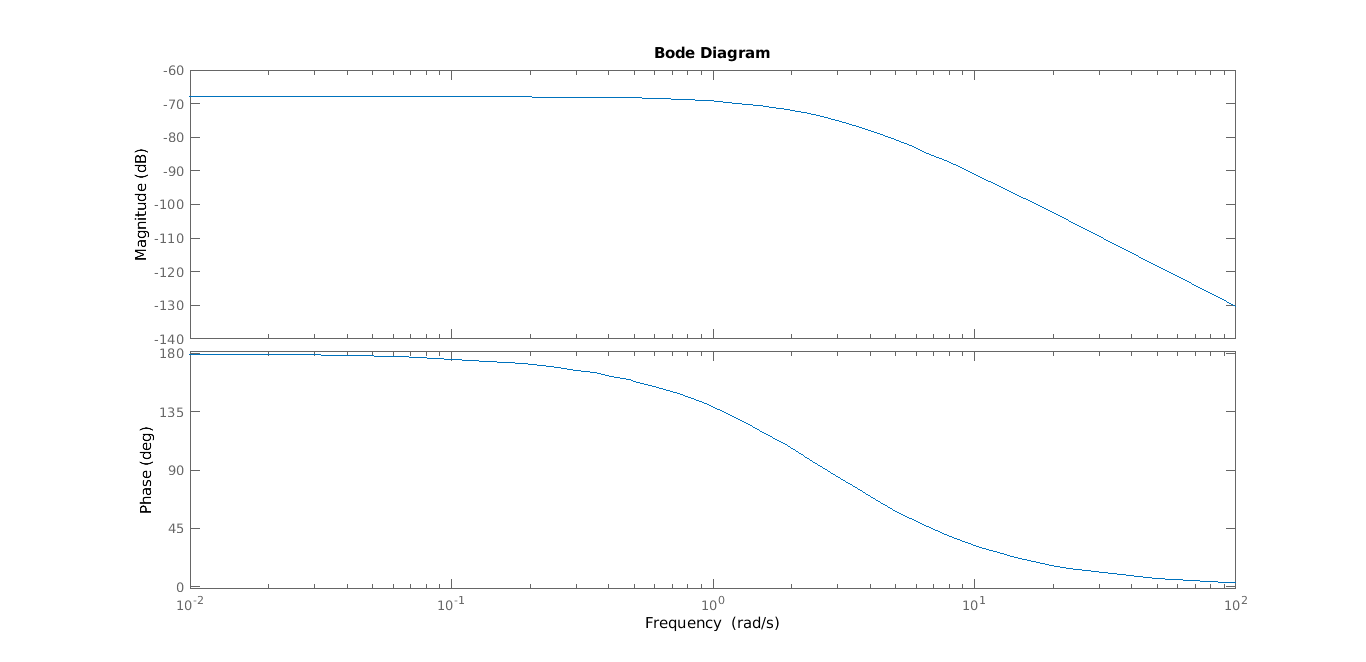
\includegraphics[width=0.9\textwidth]{manip_5_bode.png}
  \caption{Diagramme de bode système en boucle ouverte}
  \label{fig:label}
\end{figure}
\paragraph{Manip.5}
La marge de phase est nulle, on met en place un correcteur intégrale pur qui apporte stabilité et précission au système:

\begin{minted}{matlab}
Ti = 4e-4
CI =  tf(1,[-Ti 0]); % négatif pour avoir une phase >180
%bode(H,CI*H,'grid')
figure();
margin(CI*H)  
\end{minted}
\begin{figure}[H]
  \centering
  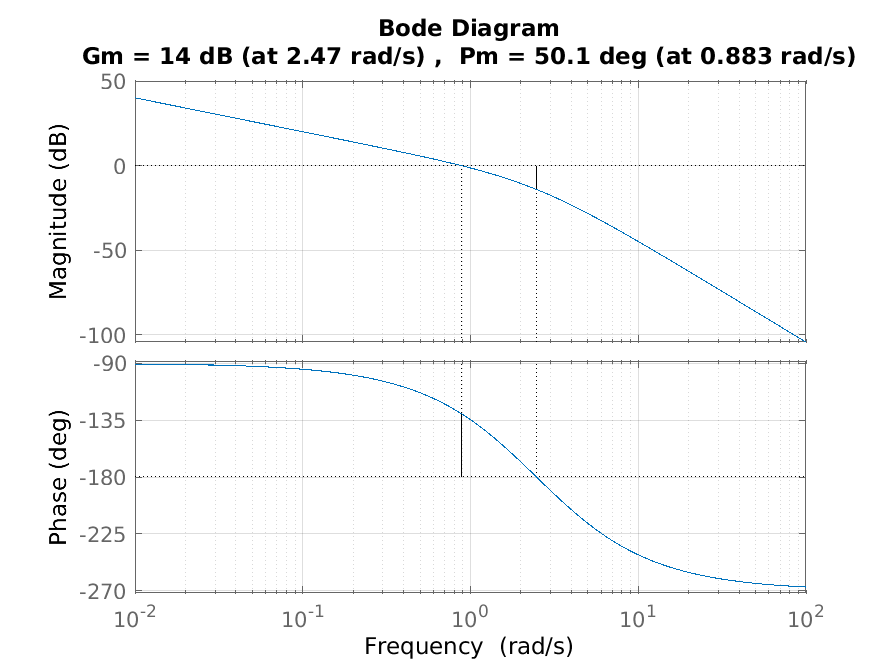
\includegraphics[width=0.7\textwidth]{manip_5marge.png}
  \caption{Marge de Phase et Gain pour $T_i=4.10^{-4}$}
  \label{fig:margin}
\end{figure}
sur la figure\ref{fig:margin} on relève une marge de phase de 50$^o$ , le cahier des charge est respecté.

\begin{figure}[ht]
  \centering
  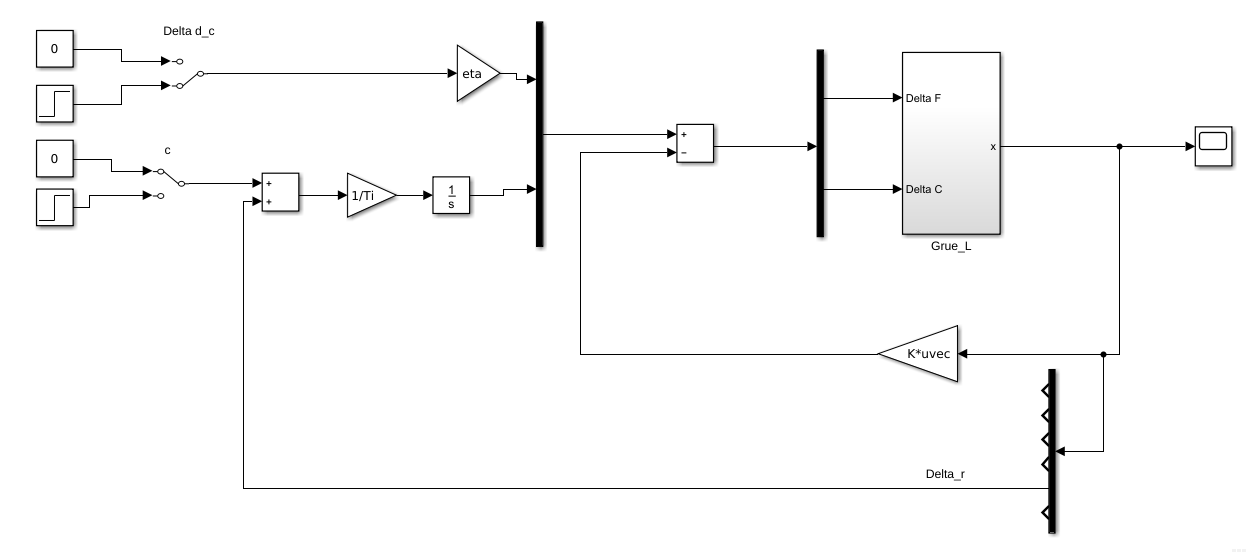
\includegraphics[width=0.9\textwidth]{bouclage_modele_L.png}
  \caption{Modèle Linéaire compléter par le correcteru par retour d'état.}
  \label{fig:label}
\end{figure}

\paragraph{Manip.6}
Avec une commande $\Delta d_c = 20$m on obtient la figure suivante:
\begin{figure}[ht]
  \centering
  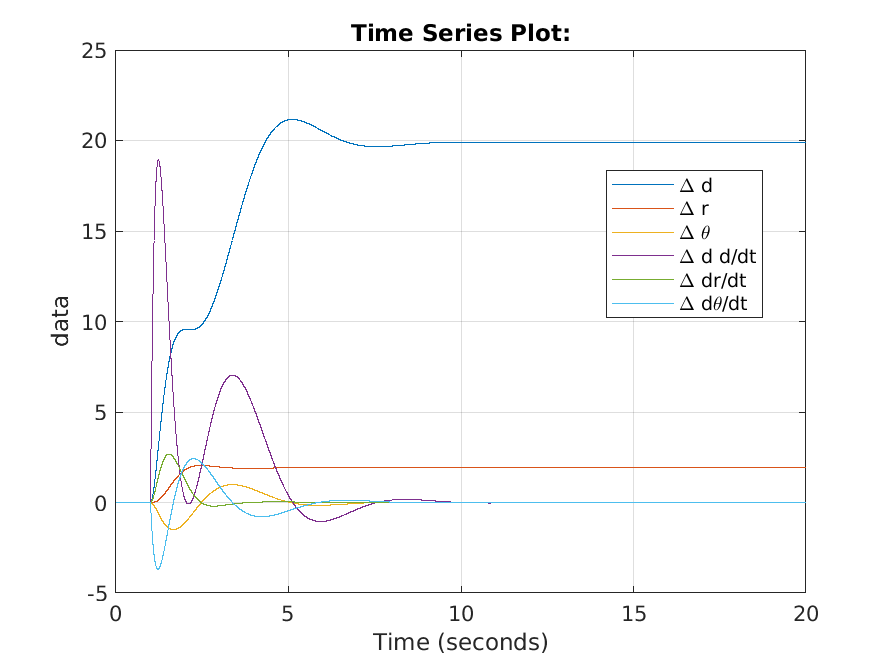
\includegraphics[width=0.7\textwidth]{manip6_20.png}
  \caption{sortie du système pour une commande de 20m}
  \label{fig:gain20}
\end{figure}

On remarque que le système n'est plus précis, il faut recaler le gain, ici manuellement, pour obtenir un système précis.
On atteint les limites du modèle linéaire, pour des commandes plus grande ou plus complexe il va falloir tenir compte des non-linéarités du système.

\paragraph{Manip.7}
On applique le correcteur au modèle non linéaire, en ayant recentrer le
retourd'état autour de son point de fonctionnement.
On obtient une sortie chaotique, mais douce. comme on peux le voir sur la figure \ref{fig:dc_var} 
\paragraph{Manip.8}
Un changement de consigne apporte un comportement différents :
\begin{figure}[H]
  \centering 
\begin{subfigure}{0.5\textwidth}
  \centering
  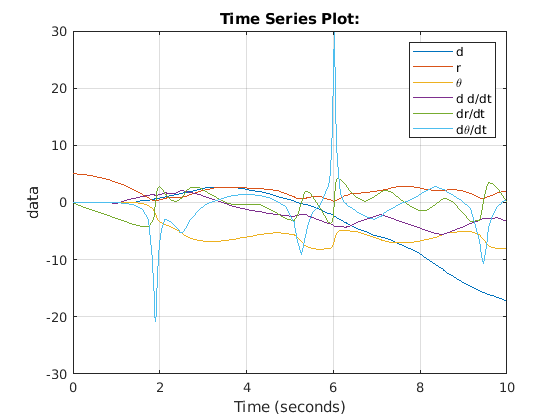
\includegraphics[width=\textwidth]{NL_correcL10.png}
  \caption{$d_c=10$}
  \label{fig:label}
\end{subfigure}%
\begin{subfigure}{0.5\textwidth}
  \centering
  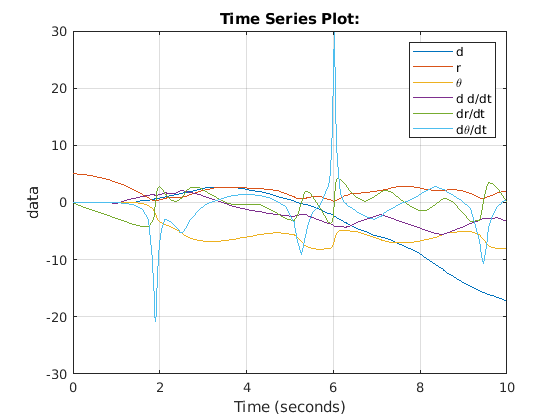
\includegraphics[width=\linewidth]{NL_correcL100.png}
  \caption{$d_c=100$}
  \label{fig:label}
\end{subfigure}\\
\begin{subfigure}{0.5\textwidth}
  \centering
  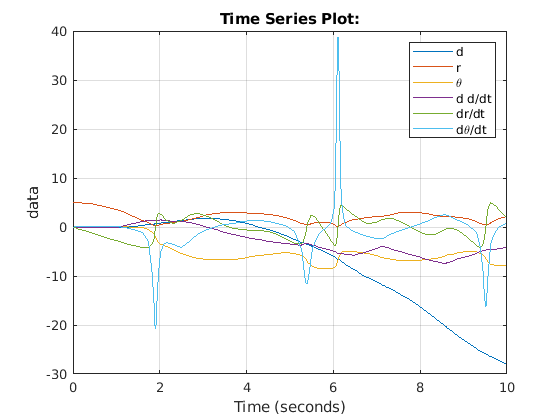
\includegraphics[width=\linewidth]{NL_correcL1.png}
  \caption{$d_c=1$}
  \label{fig:label}
\end{subfigure}
\caption{différentes sorties pour des consignes différentes}
\label{fig:dc_var}
\end{figure}






\section{Commande non linéaire hiérarchisante}
\subsection{commande à grand gain}
\paragraph{Prépa.6} On planifie la trajectoire avec:
\begin{equation}
  \begin{aligned} D_{c}(t) &=(1-\phi(t)) D_{i n i}+\phi(t) D_{f i n} \\
    R_{c}(t) &=(1-\phi(t)) R_{i n i}+\phi(t) R_{f i n}
  \end{aligned}
\end{equation}
Avec les conditions initiales et finales sur les positions
$\phi(0)=0 \quad$ et $\quad \phi(\Delta t)=1$
et celles sur la vitesse et l'accélération
$\forall i=1,2\left.\frac{d^{i} \phi(t)}{d t^{i}}\right|_{t=0}=0 \quad$ et $\quad\left.\frac{d^{i} \phi(t)}{d t^{i}}\right|_{t=\Delta t}=0$
On a 6 conditions à respecter, donc on choisit un polynôme de degré 5:
\[
  \phi(t) = a_5 t^5 + a_4 t^4 +a_3 t^3 + a_2 t^2+a_1 t+ a_0
\]

Les conditions initiales imposent  $a_0=a_1=a_2 = 0$ on a donc le polynome : $ \phi(t) = a_5 t^5 + a_4 t^4 +a_3 t^3$.
Alors :
\begin{equation}
  \begin{aligned} \alpha(\Delta t)=1 & \Rightarrow \quad a_5 \Delta t^{5} \quad+a_4 \Delta t^{4} \quad+a_3 \Delta t^{3}=1 \\
    \left.\frac{d \alpha(t)}{d t}\right|_{t=\Delta t}=0 & \Rightarrow 5 a_5 \Delta t^{4} \quad+4 a_4 \Delta t^{3}+3 a_3 \Delta t^{2}=0 \\
    \left.\frac{d^{2} \alpha(t)}{d t^{2}}\right|_{t=\Delta t}=0 & \Rightarrow 20 a_5 \Delta t^{4}+12 a_4 \Delta t^{3}+6 a_3 \Delta t^{2}=0
  \end{aligned}
\end{equation}
En résolvant le système on obtient:
\[
  a_5 = \frac{6}{\Delta t^5} ,\quad a_4 = \frac{-15}{\Delta t^4}, \quad a_3 = \frac{10}{\Delta t^3}
\]

\paragraph{Prépa.7} à partir de l'équation (2.4) de l'énoncé on a :

\begin{equation}
  \frac{1}{\omega_{0}^{2}}=\frac{R}{g} \Rightarrow \omega_{0}=\sqrt{\frac{g}{R}}
\end{equation}

\paragraph{Prépa.8} on a les commandes :
\begin{equation}
  F=\frac{M_{c}}{\epsilon_{d}}\left(\dot{D}_{c}-\dot{d}\right) \text{ et } C=-\frac{J / b+m b}{\epsilon_{r}}\left(\dot{R}_{c}-\dot{r}\right)
\end{equation}
soit le modèle :
\begin{equation}
  \dot{x}=\left[ \begin{array}{c}{\Delta d} \\ {\Delta r} \\ {\frac{m g}{M_{c}} \Delta \theta-\frac{C_{d}}{M_{c}} \Delta d+\frac{1}{\epsilon_{d}}\left(\dot{D}_{c}-\dot{d}\right)} \\ {\frac{-C_{r}}{J+m b^{2}}+\frac{F_{c}-\dot{r}}{\epsilon_{r}}} \\ {\Delta \theta}\end{array}\right]
\end{equation}
D'où :
\begin{equation}
  \begin{aligned}
    \ddot{\Delta d} &=-\left(\frac{C_{d}}{M_{c}}+\frac{1}{\epsilon_{d}}\right) \Delta d+\frac{\dot{D}_{c}}{\epsilon_{d}}+\frac{m g}{M_{c}} \Delta \theta \\
    \ddot{\Delta r} &=-\left(\frac{C_{r}}{J+m b^{2}}+\frac{1}{\epsilon_{r}}\right) \Delta r+\frac{\dot{R}_{c}}{\epsilon_{r}} \\
    \text { On peut poser } \tau_{d} &=\frac{1}{\frac{C_{d}}{M_{c}}+\frac{1}{\epsilon_{d}}} \\
    \text { et } \tau_{r} &=\frac{1}{\frac{C_{r}}{J+m b^{2}}+\frac{1}{\epsilon_{r}}}
  \end{aligned}
\end{equation}
En considérant $\epsilon_d \ll 1 $ et $\epsilon_r <<1 $ on a $\tau_d \simeq \epsilon_d$ et $\tau_r \simeq \epsilon_r$

\paragraph{Prépa.9}
On doit prendre  $\epsilon_d$ et $\epsilon_r$ suffisamment petit devant la pulsation du sytème $\omega_0$, pour avoir une commande qui puisse  compenser suffisament vite les oscillations du système.
\paragraph{Manip.9}
La commande est réalisé comme sur la figure \ref{fig:schemNL}. On
obtient alors les sorties de la figure \ref{fig:pours_traj}
\begin{figure}[H]
  \centering
  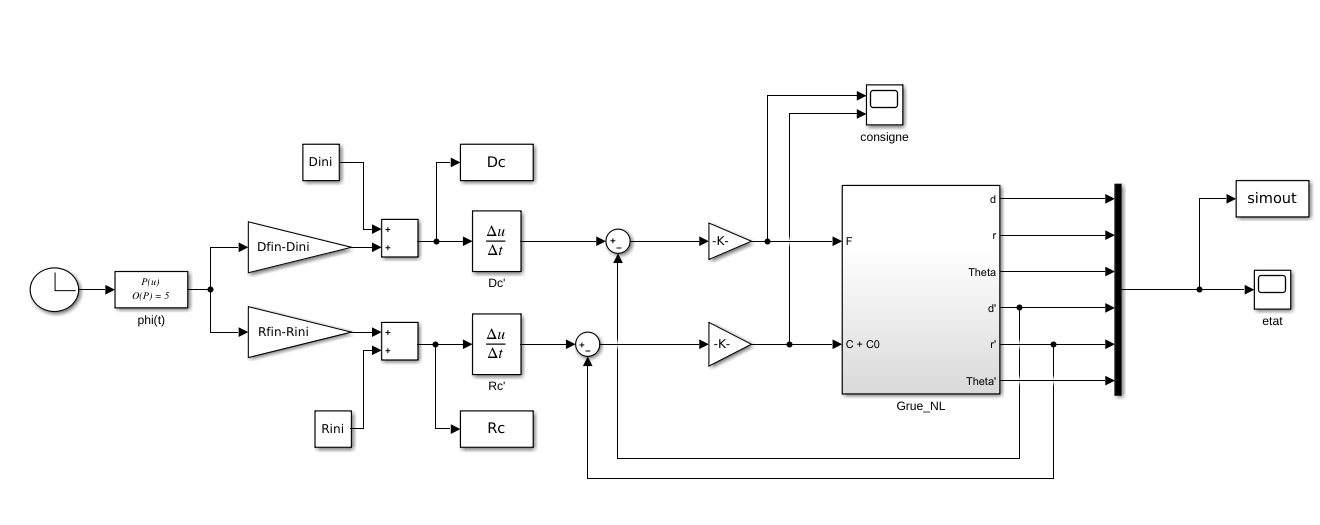
\includegraphics[width=0.9\textwidth]{boucleNL.png}
  \caption{Élaboration de la commande pour la porsuite de trajectoire}
  \label{fig:schemNL}
\end{figure}

\begin{figure}[H]
  \centering
  \begin{subfigure}{0.5\textwidth}
    \centering
    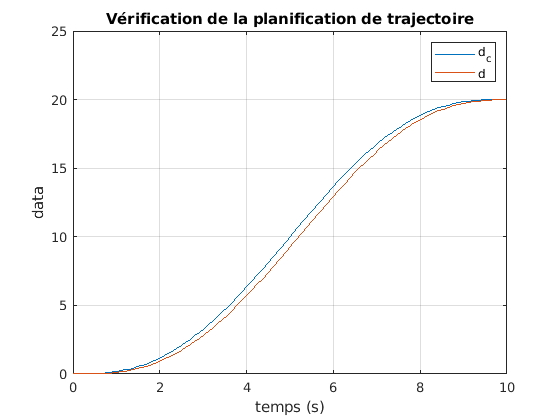
\includegraphics[width=\linewidth]{traj_plan_d}
    \caption{poursuite sur $d$}
    \label{fig:label}
  \end{subfigure}%
\begin{subfigure}{0.5\textwidth}
  \centering
  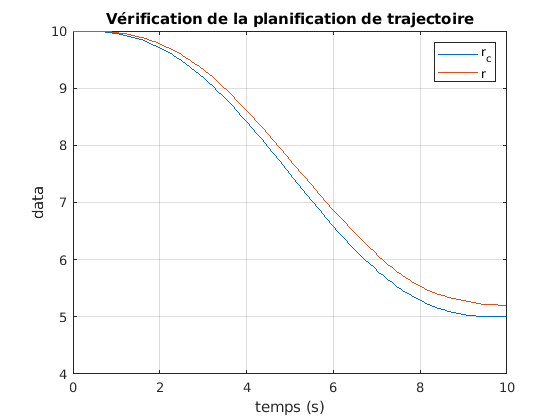
\includegraphics[width=\linewidth]{traj_plan_r}
  \caption{Poursuite sur $r$}
  \label{fig:label}
\end{subfigure}
\caption{Commande en poursuite de trajectoire}
\label{fig:pours_traj}
\end{figure}
sur la figure \ref{fig:pours_traj} on remarque que la poursuite est
plutot bien respecté pour $d$, mais celle sur $r$ conduit à un écart
final non nul , cela est d'autant plus vrai si $\epsilon_d=\epsilon_r$ devient grand comme sur la figure \ref{fig:eps}.
\begin{figure}[H]
  \centering
  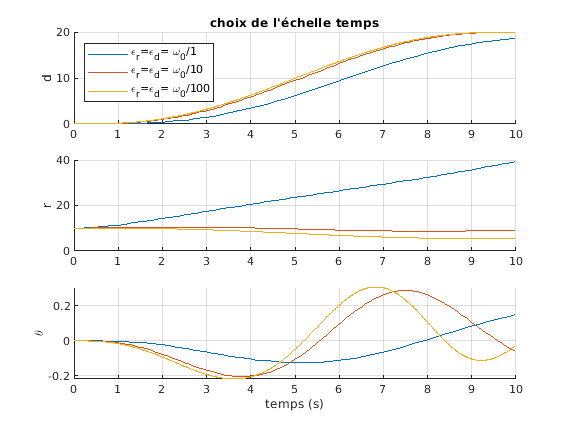
\includegraphics[width=0.7\textwidth]{eps_choix}
  \caption{Influence de $\epsilon$ sur la trajectoire réelle}
  \label{fig:eps}
\end{figure}

\paragraph{Manip.10}
On fait varier la masse dans la synthèse de l'asservissement, en ayant choisi
$\epsilon_d=\epsilon_r= \omega_0/100$.
\begin{figure}[H]
  \centering
  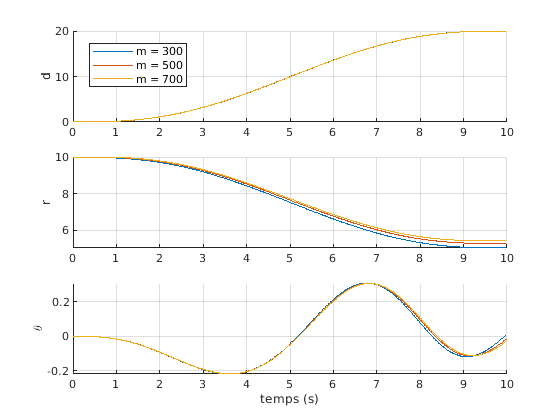
\includegraphics[width=0.7\textwidth]{m_choix}
  \caption{Robustesse face à une pertubation de la masse}
  \label{fig:m_choix}
\end{figure}
On remarque qu'une variation de 200kg n'entraine qu'un écart d'une 30aine de
centimètre avec la consigne ce qui est largement acceptable.


\paragraph{Manip.11}
En étudiant des variation sur $C_r$ et $C_d$ on ne remarque aucun changement
pour $\epsilon = \omega_0/100$ ou  $\epsilon = \omega_0/10$.

La commande suivant le modèle précédement décrit est donc très robuste
aux pertubations , tant que sa dynamique est rapide devant celle du système.

\subsection{Platitude}
\paragraph{Prépa.10}
On montre d'abords que le système est plat pour les sorties $(x, z),$
\begin{equation}
  \left\{
    \begin{aligned}
      x &=r \sin \theta+d \\
      m \ddot{x} &=-T \sin \theta
    \end{aligned}
  \right. \Rightarrow d=x+r \frac{m \ddot{x}}{T}
\end{equation}

Or on a:
\begin{equation}
  \begin{cases}
    m \ddot{x}=-T \sin \theta \\
    m \ddot{z}=-T \cos \theta+m g
  \end{cases} \Rightarrow T=m \sqrt{\ddot{x}^{2}+(g-\ddot{z})^{2}}
\end{equation}
\begin{equation}
  \begin{cases}
    x=r \sin \theta+d \\
    z=r \cos \theta
  \end{cases} \Rightarrow r^{2}=(x-d)^{2}+z^{2}
\end{equation}
Soit :
\begin{equation}
  \begin{cases}
    x-d &=-r \frac{m \ddot{x}}{T} \\
    r^{2} &=(x-d)^{2}+z^{2}
  \end{cases} \Rightarrow r^{2}=\frac{z^{2}}{1-\frac{\ddot{x}^{2}}{\vec{x}^{2}+(g-\ddot{z})^{2}}}
\end{equation}

Or $\theta = \arccos{\frac{z}{r}}$ on a donc :

\begin{equation}
r=\sqrt{\frac{z^{2}}{1-\frac{\ddot{x}^{2}}{\ddot{x}^{2}+(g-\ddot{z})^{2}}},}, d=x+\sqrt{\frac{z^{2}}{(g-\ddot{z})^{2}}} \ddot{x}, \quad \text { et } \theta=\arccos \sqrt{1-\frac{\ddot{x}^{2}}{\ddot{x}^{2}+(g-\ddot{z})^{2}}}
\end{equation}
Les variables d'états de dépendent donc que des sorties et de leurs dérivées, de même pour la commande 
\begin{equation}
  \begin{aligned}
    C &=b T-C_{r} \frac{\dot{r}}{b}-J \frac{\ddot{r}}{b} \\
    F &=M_{c} \ddot{d}-T \sin \theta+C_{d} \dot{d}
  \end{aligned}
\end{equation}
Le système est plat ,avec le sorties  plates $x,z$
\paragraph{Prépa.11}
Les conditions imposées sont :
\begin{equation}
  \begin{cases}
    d(t=0) = D_{ini} \\
    r(t=0) = R_{ini} \\
    \theta(t=0) = 0
  \end{cases} \quad\text{ et }\quad
  \begin{cases}
    d(t=\Delta t ) = D_{fin} \\
    r(t=\Delta t ) = R_{fin} \\
    \theta(t=\Delta t ) = 0
  \end{cases}
\end{equation}
Ce qui se transpose aux coordonnées:
\begin{equation}
  \begin{cases}
    x(t=0) = D_{ini}\\
    z(t=0) = R_{ini} \\
  \end{cases} \quad\text{ et }\quad
  \begin{cases}
    x(t=\Delta t) = D_{fin}\\
    z(t=\Delta t) = R_{fin} \\
  \end{cases}
\end{equation}

On pose donc :
\begin{equation}
  \begin{aligned}
    x_{c}(t) &=(1-\phi_2(t)) D_{i n i}+\phi_2(t) D_{f i n} \\
    z_{c}(t) &=(1-\phi_2(t)) R_{i n i}+\phi_2(t) R_{f i n}
  \end{aligned}
\end{equation}
De manière analogue à la préparation 6 on a les conditions initiales et finales sur les positions  et leur dérivées:
\[
  \phi_2(0) = 0 ,\quad \phi_2(\Delta t) =1, \quad \forall i = 1,2,3\left. \deriv[^i\phi_2(t)]{t^i}\right|_{t=0}= 0 \text{ et } \left.\deriv[^i\phi_2(t)]{t^i}\right|_{t=\Delta t}= 0
\]
Pour satisfaire les 8 conditions on choisit un polynome d'ordre 7 :
\begin{equation}
  \phi_2(t)=a_{7} t^{7}+a_{6} t^{6}+a_{5} t^{5}+a_{4} t^{4}+a_{3} t^{3}+a_{2} t^{2}+a_{1} t+a_{0}
\end{equation}
Les conditions initiales imposent $a_0=a_1=a_2=a_3 =0$ et les conditions finales donnent :
\begin{equation}
  \begin{array}{llllll}
    \phi_2(\Delta t)                                          & =1 =  & a_7\Delta t^7    & + a_6 \Delta t^6  & + a_5 \Delta t^5 & + a_4 \Delta t^4 \\[1em]
    \left.\frac{d \phi_2(t)}{d t}\right|_{t=\Delta t}         & =0 =  & 7a_7\Delta t^6   & + 6a_6 \Delta t^5 &+ 5a_5\Delta t^4   &+ 4a_4 \Delta t^3  \\[1em]
    \left.\frac{d^{2} \phi_2(t)}{d t^{2}}\right|_{t=\Delta t} & =0 =  & 42a_7\Delta t^5  & +30a_6 \Delta t^4 &+ 20a_5 t^3   &+ 12a_4\Delta t^2  \\[1em]
    \left.\frac{d^{3} \phi_2(t)}{d t^{3}}\right|_{t=\Delta t} & =0  = & 210a_z\Delta t^4 & +120a_6\Delta t^3 &+ 60a_5 \Delta t^2 &+ 24a_4\Delta t 
  \end{array}
\end{equation}
On a donc :
\begin{equation}
  a_{7}=\frac{-20}{\Delta t^{7}}, \quad a_{6}=\frac{70}{\Delta t^{6}}, \quad a_{5}=\frac{-84}{\Delta t^{5}}, \quad a_{4}=\frac{35}{\Delta t^{4}}
\end{equation}

\paragraph{Prépa.12}

On impose une trajectoire parabolique ainsi,au niveau niveau de l'obstacle :$x_c=x_H \implies z_c=z_H$. On pose donc :
\[
  z_c = a(x_c-x_h)^2+z_h
\]
En évaluant cette expression à la position initiale on a:
\[
  a = \frac{R_{ini}-z_H}{(D_{ini}-x_H)^2}
\]
Pour déterminer $x_H$ on utilise la position finale et on a:

\begin{equation}
  x_{H}=\frac{D_{i n i}+\sqrt{\frac{R_{i n i}-z_{H}}{R_{i n i}-z_{H}}} D_{f i n}}%
{1+\sqrt{\frac{R_{i n i}-z_{H}}{R_{f i n}-z_{H}}}}
\end{equation}
\paragraph{Manip.12}
Cette fois ci on utilise les sorties plates, et on a donc :
\[
  \begin{cases}
    \dot{D_c}(t) &= \displaystyle\deriv[]{t}\left( x_c- \frac{\ddot{x_c}z_c }{\ddot{z_c}-g}\right)\\
    \dot{R_c}(t) &= \displaystyle\deriv[]{t}\sqrt{z_c^2-\left(\frac{\ddot{x_c}z_c }{\ddot{z_c}-g}\right)^2}
  \end{cases}
\]
On construit alors les différents blocs de synthèse de la commande par
sortie plates:
\begin{figure}[H]
  \centering
  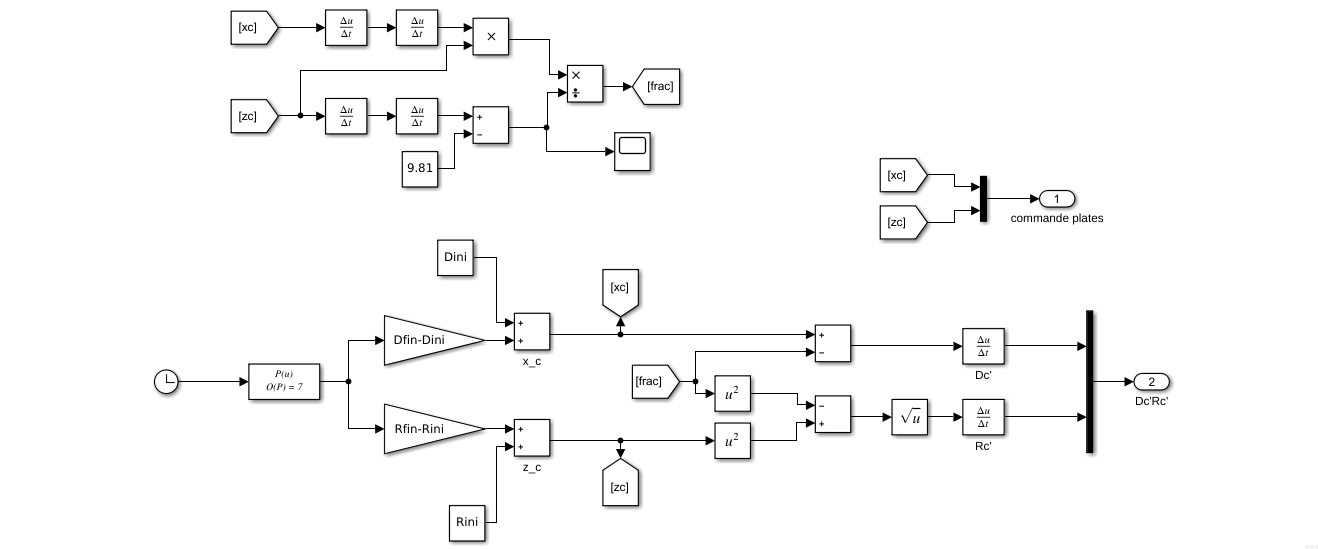
\includegraphics[width=0.7\textwidth]{rect_plat.png}
  \caption{Synthèse de la trajectoire rectiligne par sortie plate}
  \label{fig:label}
\end{figure}On obtient alors les resultats suivant sur la commande des sorties
plates (figure \ref{fig:sortiesplates}).\\

\textit{Remarque}: Pour mener la simulation a bien il a fallut
modifier les paramètres d'intégrations (pas fixe de 1e-4, méthode
d'Euler) qui influait sur la régularité des sorties et commmandes.
\begin{figure}[H]
  \centering
  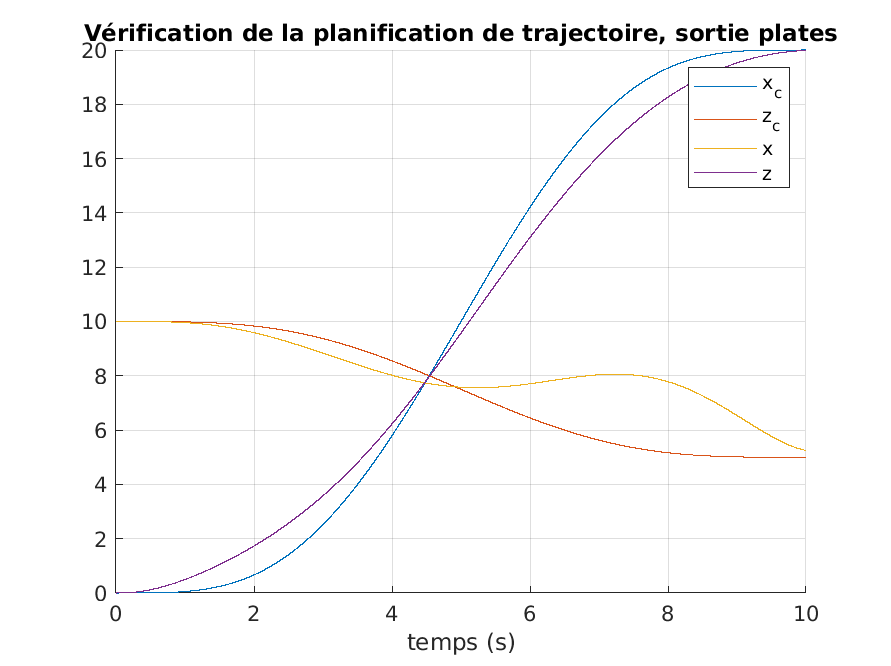
\includegraphics[width=0.7\textwidth]{manip12.png}
  \caption{Sorties plates commandées, $\epsilon= \omega_0/100$}
  \label{fig:sortiesplates}
\end{figure}


\paragraph{Manip.13}
De meme on mets en place la synthèse de la parabole de commande
\begin{figure}[H]
  \centering
  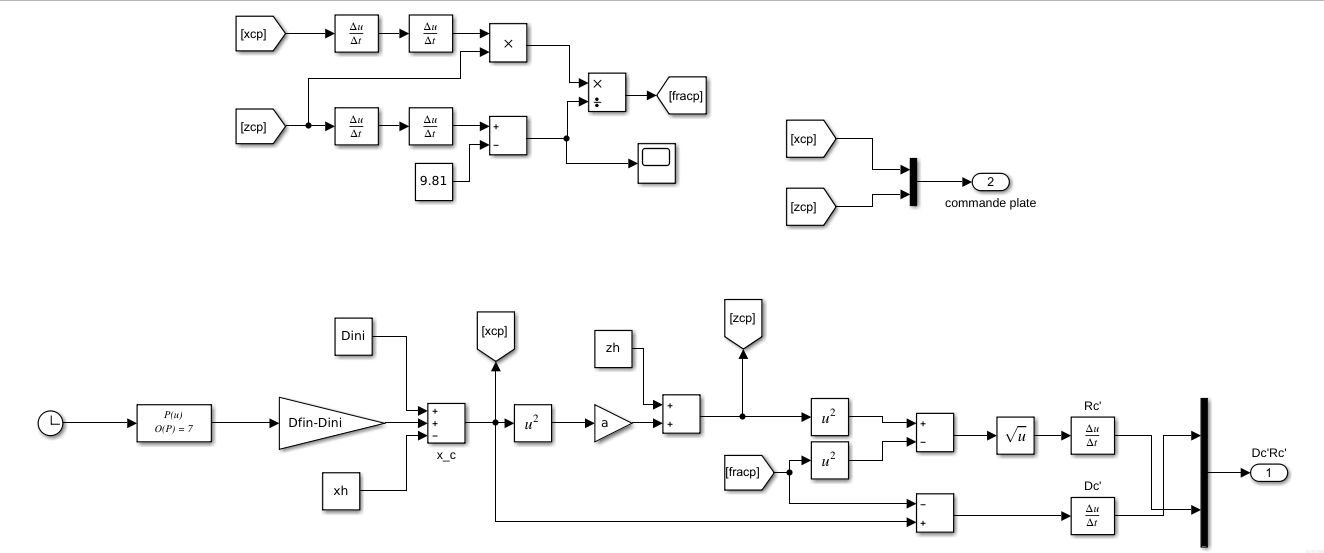
\includegraphics[width=0.9\textwidth]{sortie_plate.png}
  \caption{Synthèse des sorties plates}
  \label{fig:label}
\end{figure}

On obtient alors les resultats suivants sur la commande des sorties
plates (figure \ref{fig:sortiesplates}).\\

\textit{Remarque}: Meme paramètres d'intégration que précédement
\begin{figure}[H]
  \centering
  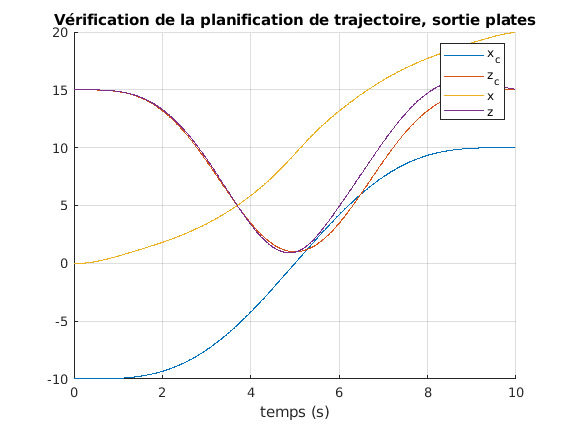
\includegraphics[width=0.9\textwidth]{manip13e100.png}
  \caption{Sorties plates commandé en parabole}
  \label{fig:sortiesplates}
\end{figure}

Les resultats sont peux satisfaisant,mais la consigne est globalement
respectée, il faudrait investiguer plus en profondeur la modélisation
réalisée et comparée avec la commande du système réel, ce qui n'a pu
être fait par manque de temps.

\section*{Conclusion}
Dans ce TP nous avons modélisé le système présenté d'abord de manière
linéaire, ce qui ne s'est pas avéré assez suffisant pour des commandes
qui nous faisait sortir de la plage de linéarisation. En prenant en
compte les non-linéarités on peux commander de manière plus précise et
plus robuste le modèle, et réaliser une poursuite de trajectoire
correcte. Avec l'utilisation des sorties plates on a pu aller plus on
simulant le contournement d'un obstacle.
\end{document}

%%% Local Variables:
%%% mode: latex
%%% TeX-master: t
%%% End:
